\chapter{The Compost Bomb and the Terrestrial Carbon Cycle}
\graphicspath{{global_bomb/figs/}}

\todo[inline]{This is basically just going to be equations for now}

Following\cite{Luke2011}, we have the compost comb equations
\begin{subequations}
  \label{eq:compost_bomb_equations}
  \begin{align}
    \mu \dv{T_s}{t} &= - \kappa \left(T_s - T_a\right) + Ar_0C_se^{\alpha T_s} \label{eq:compost_bomb_soil_temperature} \\
    \dv{C_s}{t} &= \Pi - r_0C_se^{\alpha T_s} \label{eq:compost_bomb_soil_carbon}
  \end{align}
\end{subequations}

Noting the obvious timescale seperation in \cref{eq:compost_bomb_equations} we can put \cref{eq:compost_bomb_soil_temperature} into
equilibrium to get
\begin{equation*}
  0 = - \kappa \left(T_s - T_a\right) + Ar_0C_se^{\alpha T_s}
\end{equation*}
which can be solved for the soil temperature to  give
\begin{equation}
  \label{eq:soil_temperature_equilibrium}
  T_s = T_a - \frac{1}{\alpha} W\left(-\frac{Ar_0C_s \alpha e^{\alpha T_a}}{\kappa} \right),
\end{equation}
where $W(x)$ is the Lambert $W$ function. The Lambert $W$ function is defined as the solution to the equation
\begin{equation}
  \label{eq:lambert_W}
  W(x)e^{W(x)} = x.
\end{equation}

\begin{figure}
  \centering
  \begin{tikzpicture}
    \begin{axis}[
      xmin=-1,
      xmax=4,
      enlarge y limits=false,
      axis lines=left,
      xlabel=$x$,
      ylabel=$W(x)$,
      samples=50]
      \addplot[domain=-5:-1] (x * exp(x), x);
      \addplot[domain=-1:2] (x * exp(x), x);
    \end{axis}
  \end{tikzpicture}
  \caption{The Lambert $W$ function}
  \label{fig:lambert_W}
\end{figure}
The Lambert $W$ is plotted in \cref{fig:lambert_W}.

Defining
\begin{equation}
  \label{eq:critical_npp}
  \Pi_c = \frac{\kappa}{\alpha A}
\end{equation}
we can rewrite \cref{eq:soil_temperature_equilibrium} as
\begin{equation}
  \label{eq:soil_temperature_equilibrium_nppc}
  T_s = T_a - \frac{1}{\alpha} W\left(-\frac{r_0C_s e^{\alpha T_a}}{\Pi_c} \right).
\end{equation}
We should therefore insert \cref{eq:soil_temperature_equilibrium_nppc} in \cref{eq:compost_bomb_soil_carbon}
to give
\begin{equation}
  \label{eq:soil_carbon_evolution}
  \dv{C_s}{t} = \Pi + \Pi_c W\left(-\frac{r_0C_s e^{\alpha T_a}}{\Pi_c} \right).
\end{equation}
This implies the equilibrium value of $C_s$ is
\begin{equation}
  \label{eq:equilibirum_soil_carbon}
  C_s^{\mathrm{eq}} = \frac{\Pi}{r_0} e^{-\alpha T_a} e^{-\Pi/\Pi_c}.
\end{equation}
Note that we recover the no biogeochemcial heating case by sending $\Pi_c \rightarrow \infty$.


Recognising that
\begin{equation}
  \label{eq:atmospheric_temperatures}
  T_a = \frac{S}{\log 2} \log \frac{C_a}{C_{a0}} 
\end{equation}
leads, upon substituting \cref{eq:atmospheric_temperatures} into \cref{eq:soil_carbon_evolution},
\begin{equation}
  \label{eq:global_soil_carbon}
  \dv{C_s}{t} = \Pi + \Pi_c W\left(-\frac{r_0C_s}{\Pi_c} \left(\frac{C_a}{C_{a0}}\right)^\mu \right),
\end{equation}
where
\begin{equation}
  \label{eq:mu}
  \mu = \frac{\alpha S}{\log 2}.
\end{equation}
We will assume
\begin{equation}
  \label{eq:npp_fertilization}
  \Pi(C_a) = \Pi_{\infty}\frac{C_a}{C_a + C_{a_{1/2}}}.
\end{equation}
We will assume further that a fixed fraction $\chi_0$ of atmospheric emissions reaches the ocean, meaning
\begin{equation}
  \label{eq:simple_ocean}
  C_a = C_{a0} -\frac{1}{1+\chi_0} (C_s - C_{s}^{\mathrm{eq}})
  %C_s = C_{s}^{\mathrm{eq}} - (1 + \chi_0)(C_a - C_{a0}.
\end{equation}
We chose the temperature anomaly so that $T_a = 0$ corresponds to an equilibrium. We can then set
$r_0 = \frac{\Pi}{C_s^{\mathrm{eq}}}e^{-\Pi/\Pi_c}$ giving
\begin{equation}
  \label{eq:soil_carbon_evolution_with_r0_fixed}
  \dv{C_s}{t} = \Pi + \Pi_c W\left(-\frac{C_s}{C_s^{\mathrm{eq}}}\frac{\Pi}{\Pi_c}e^{-\Pi/\Pi_c} \left(\frac{C_a}{C_{a0}}\right)^\mu \right).
\end{equation}

To find the bifurcation we therefore just have to calculate where
\begin{equation*}
  \dv{\dot{C_s}}{t} = 0,
\end{equation*}
we will make use of
\begin{equation}
  \label{eq:derivative_of_lambert_W}
  W'(x) = \frac{W(x)}{x\left(1 + W\left(x\right)\right)}.
\end{equation}
This leads to
\begin{equation}
  \label{eq:critical_mu}
  \mu^* = \left(1 + \chi_0\right) \frac{C_{a0}}{C_s^{\mathrm{eq}}} \left(1+\frac{1}{1+\chi_0}\left( \frac{1}{W\left(-\frac{\Pi}{\Pi_c}e^{-\Pi/\Pi_c}\right)}
      - \frac{\Pi_c}{\Pi}\right)\frac{C_s^{\mathrm{eq}}}{\Pi_c}\dv{\Pi}{C_a}\right)
\end{equation}
where $\mu^*$ is the value of $\mu$ where the bifurcation takes place.

Taking the limit as $\Pi_c \rightarrow \infty$ using the fact that $W(x) = x + \mathcal{O}(x^2)$ as $x \rightarrow 0$ gives
\begin{equation}
  \label{eq:critical_mu_no_biogeochemical}
  \mu^*_{\infty} = \left(1 + \chi_0\right) \frac{C_{a0}}{C_s^{\mathrm{eq}}} \left(1 - \frac{2}{1+\chi_0}\frac{C_s^{\mathrm{eq}}}{\Pi}\dv{\Pi}{C_a}\right).
\end{equation}

We can plot \cref{eq:critical_mu} to devide the parameter plane into a stable and unstable region.

\begin{figure}
  \centering
  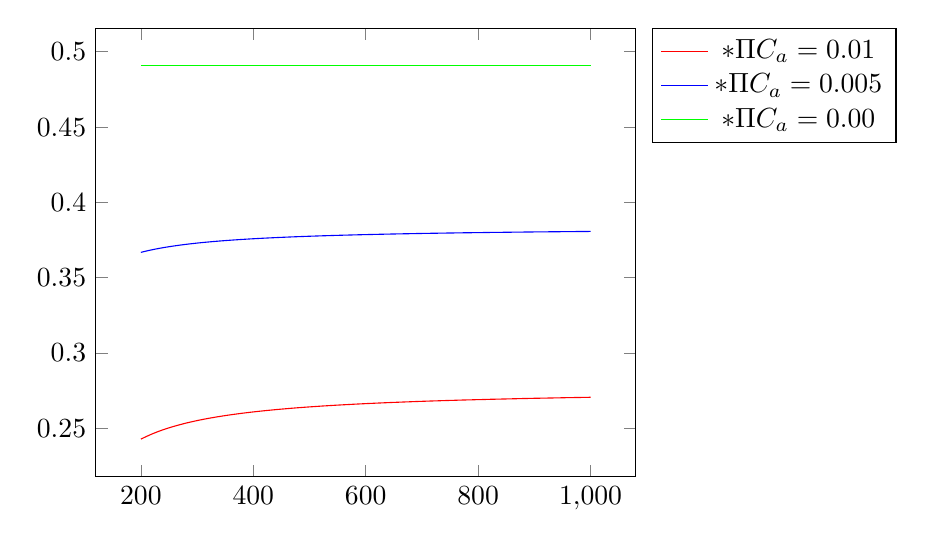
\begin{tikzpicture}[
    /pgf/declare function={
      chi0 = 0.25;
      npp = 55.0;
      Ca0 = 589.0;
      Cseq = 1500.0;
    }
    ]
    \begin{axis}[
      legend pos=outer north east,
      %enlargelimits=false
      ]
      \addplot[
      domain=200:1000,
      samples=100,
      enlarge x limits=false,
      color=red]
      {(1 + chi0)*(Ca0/Cseq)*(1 + (1/(1+chi0)) *(-1/(exp(-npp/x) * npp/x) - x/npp) * (Cseq / x) * 0.01)};
      \addlegendentry{$\dv*{\Pi}{C_a} = 0.01$}
      \addplot[
      domain=200:1000,
      samples=100,
      enlarge x limits=false,
      color=blue]
      {(1 + chi0)*(Ca0/Cseq)*(1 + (1/(1+chi0)) *(-1/(exp(-npp/x) * npp/x) - x/npp) * (Cseq / x) * 0.005)};
      \addlegendentry{$\dv*{\Pi}{C_a} = 0.005$}
      \addplot[
      domain=200:1000,
      samples=100,
      enlarge x limits=false,
      color=green]
      {(1 + chi0)*(Ca0/Cseq)*(1 + (1/(1+chi0)) *(-1/(exp(-npp/x) * npp/x) - x/npp) * (Cseq / x) * 0.00)};
      \addlegendentry{$\dv*{\Pi}{C_a} = 0.00$}

    \end{axis}
 
    
  \end{tikzpicture}
  \caption{The parameter plane}
  \label{fig:critical_mu_vs_pic}
\end{figure}\todo{check \cref{fig:critical_mu_vs_pic}}


Using \cref{eq:critical_mu_no_biogeochemical} gives an upper limit on the strength of \ce{CO2} fertilization compatible with a stable climate
\begin{equation}
  \label{eq:maximum_co2_fertilization}
  \dv{\Pi}{C_a} < \frac{1+\chi_0}{2} \frac{\Pi}{C_s^{\mathrm{eq}}} - \frac{1}{2} \frac{\Pi}{C_{a0}} \mu_{\infty}^*
\end{equation}

\begin{figure}
  \centering
  \begin{tikzpicture}[
    /pgf/declare function={
      chi0 = 0.25;
      npp = 55.0;
      Ca0 = 589.0;
      Cseq = 1500.0;
    }
    ]
    \begin{axis}[
      xlabel = $\mu$,
      ylabel = $\dv{\Pi}{C_a}$ \unit{\per\year},
      ymin=0.0,
      ymax=2.5E-2,
      xmin=0.0
      ]
      \addplot[domain=0:0.6] {0.5*(1+chi0) * npp/Cseq - 0.5 * npp * x / Ca0};
    \end{axis}
    \end{tikzpicture}
  \caption{Maximum \ce{CO2} fertilization strength}
  \label{fig:maximum_co2_fertilization}
\end{figure}